\documentclass{beamer}
\usepackage{framed}
\usepackage{graphicx}

\begin{document}
\section{Section 1 : Algorithms}
%==================================%
\begin{frame}
	\frametitle{Algorithms}
	\large
	\begin{itemize}
		\item Algorithm is a step by step procedure, which defines a set of instructions to be executed in certain order to get the desired output.
		\item Algorithms are generally created independent of underlying languages, i.e. an algorithm can be implemented in more than one programming language.
		
	\end{itemize}
	
\end{frame}
%==================================%
\begin{frame}
\noindent \textbf{(Not Examinable)}\\
From data structure point of view, following are some important categories of algorithms −
	
	\begin{description}
		\item[Search] − Algorithm to search an item in a datastructure.
		\item[Sort] − Algorithm to sort items in certain order
		\item[Insert] − Algorithm to insert item in a datastructure
		\item[Update] − Algorithm to update an existing item in a data structure
		\item[Delete] − Algorithm to delete an existing item from a data structure
	\end{description}
	
\end{frame}
%=====================================%
\begin{frame}
\frametitle{Characteristics of an Algorithm}
	Not all procedures can be called an algorithm. An algorithm should have the below mentioned characteristics −
	\begin{description}
		\item[Unambiguous] − Algorithm should be clear and unambiguous. Each of its steps (or phases), and their input/outputs should be clear and must lead to only one meaning.
		
		
		\item[Input] − An algorithm should have 0 or more well defined inputs.
		
		\item[Output] − An algorithm should have 1 or more well defined outputs, and should match the desired output.
	\end{description}
\end{frame}
%=====================================%
\begin{frame}
	\frametitle{Characteristics of an Algorithm}		
	\begin{description}
		\item[Finiteness] − Algorithms must terminate after a finite number of steps.
		
		\item[Feasibility] − Should be feasible with the available resources.
		
		\item[Independent] − An algorithm should have step-by-step directions which should be independent of any programming code.
	\end{description}
\end{frame}
%==========================================================================%
\subsection{1A - Brute Force and Combinatorial explosion}
\begin{frame}
	\frametitle{Brute Force Search}
	\begin{itemize}
		\item The brute-force search or exhaustive search, also known as generate and test, is a very general problem-solving technique that consists of systematically enumerating all possible candidates for the solution and checking whether each candidate satisfies the problem's statement.
	\end{itemize}
\end{frame}


\begin{frame}
	\frametitle{Set Theory Revision: The Power Set}
	The Power Set is the set of all possible subsets of a set. If there are $n$ elements in the set, then there are $2^n$ elements in the power set.
	\[ \{A,B,C,D,E\}\]
\end{frame}
\section{Combinatorial Explosion}

\begin{frame}
	\frametitle{Combinatorial Explosion}
	\large
	\begin{itemize}
		\item 	Combinatorial explosion is a fundamental problem in computing. 
		\item It is the problem that the number of combinations that one has to examine grows exponentially, so fast that even the fastest computers will require an intolerable amount of time to examine them.
		
	\end{itemize}
\end{frame}
%%======================================================= %
%\begin{frame}
%	\frametitle{Combinatorial explosion}
%	\begin{itemize}
%		\item The main disadvantage of the brute-force method is that, for many real-world problems, the number of natural candidates is prohibitively large. For instance, if we look for the divisors of a number as described above, the number of candidates tested will be the given number n. 
%%		\item So if n has sixteen decimal digits, say, the search will require executing at least 1015 computer instructions, which will take several days on a typical PC. If n is a random 64-bit natural number, which has about 19 decimal digits on the average, the search will take about 10 years.
%		\item  This steep growth in the number of candidates, as the size of the data increases, occurs in all sorts of problems. 
%	\end{itemize}
%	
%\end{frame}





\begin{frame}
\frametitle{Combinatorial Explosion}
\large
\begin{itemize}
	\item 	The combinatorial explosion problem limits the ability of computers to solve large problems. This is because in most realistic problems of interest to us, the number of combinations is typically very large.
	
	\item Suppose you have $n$ decisions to make and for each decision, you have 10 possible options. Then you will have all together 10 to the power n combinations of solutions. The number of combinations grows exponentially as n increases.
	\item (Binary Integer Problems - Trying by Brute Force : $2^n$ possible outcomes)
\end{itemize}	

	
	
\end{frame}
%======================================================= %
\section{Divide and Conquer}
\begin{frame}
	\Large
	\noindent \textbf{Divide and Conquer}
	\begin{figure}
		\centering
		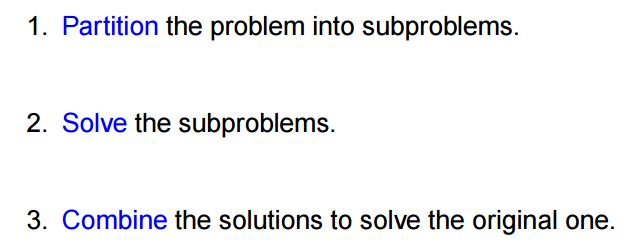
\includegraphics[width=0.9\linewidth]{divideandconquer}
		
	\end{figure}
	
\end{frame}
%==================================%
\begin{frame}
	\frametitle{Divide and Conquer}
	\large
	Broadly, we can understand divide-and-conquer approach as three step process.
	\begin{description}
		\item[Divide/Break] This step involves breaking the problem into smaller sub-problems. \\ Sub-problems should represent as a part of original problem. This step generally takes recursive approach to divide the problem until no sub-problem is further dividable. \\ At this stage, sub-problems become atomic in nature but still represents some part of actual problem.
	\end{description}
	
\end{frame}
%==================================%
\begin{frame}
	\frametitle{Divide and Conquer}
	\large
	\begin{description}
		\item[Conquer/Solve]
		This step receives lot of smaller sub-problem to be solved. \\ Generally at this level, problems are considered 'solved' on their own.
		\medskip
		\item[Merge/Combine]
		When the smaller sub-problems are solved, this stage recursively combines them until they formulate solution of the original problem.
	\end{description}
\end{frame}
%======================================================= %
\section{Greedy Algorithms}

%- http://www.cs.princeton.edu/~wayne/kleinberg-tardos/pdf/04GreedyAlgorithmsI.pdf
%- https://www.hackerearth.com/practice/algorithms/greedy/basics-of-greedy-algorithms/tutorial/

%==================================================================%
\begin{frame}
	\frametitle{Greedy Algorithm}
	
	\large
	
	%- http://www.personal.kent.edu/~rmuhamma/Algorithms/MyAlgorithms/Greedy/greedyIntro.htm
	\begin{itemize}
		\item 	Greedy algorithms are simple and straightforward. They are shortsighted in their approach in the sense that they take decisions on the basis of information at hand without worrying about the effect these decisions may have in the future. 
		\item They are easy to invent, easy to implement and most of the time quite efficient. Many problems cannot be solved correctly by greedy approach. 
		\item Greedy algorithms are used to solve optimization problems
	\end{itemize}

	
	
\end{frame}
%===============================%
\begin{frame}
	\frametitle{Greedy Algorithm}
	
	\begin{framed}
	\textbf{Greedy Approach:} Greedy Algorithm works by making the decision that seems most promising at any moment; it never reconsiders this decision, whatever situation may arise later.
	\end{framed}
	

	As an example consider the problem of "Making Change". The coins available are:
	
	\begin{itemize}
		\item dollars (100 cents)
		\item quarters (25 cents)
		\item dimes (10 cents)
		\item nickels (5 cents)
		\item pennies (1 cent)
	\end{itemize}

	
	

	
\end{frame}
%===============================%
\begin{frame}
	\frametitle{Greedy Algorithm} 
	
\textbf{ (Not Examinable) Example }  
	\begin{itemize}
	\item  Make a change for 2.89 (289 cents) here n = 2.89 and the solution contains 2 dollars, 3 quarters, 1 dime and 4 pennies. 
	\item The algorithm is greedy because at every stage it chooses the largest coin without worrying about the consequences.
	\item  Moreover, it never changes its mind in the sense that once a coin has been included in the solution set, it remains there.
	\end{itemize}
	
	
\end{frame}
%===============================%
\begin{frame}
	\frametitle{Greedy Algorithm}
\noindent \textbf{Problem:}  Make a change of a given amount using the smallest possible number of coins. \\ \medskip
	
\noindent \textbf{Informal Algorithm}
	\begin{itemize}
		\item Start with nothing.
		\item at every stage without passing the given amount.
		\item add the largest to the coins already chosen.
	\end{itemize}
	

	
	
\end{frame}
%===============================%
%\begin{frame}
%	\frametitle{Greedy Algorithm}
%	
%	Formal Algorithm
%	
%	Make change for n units using the least possible number of coins.
%	
%	MAKE-CHANGE (n)
%	C ← {100, 25, 10, 5, 1}     // constant.
%	Sol ← {};                         // set that will hold the solution set.
%	Sum ← 0 sum of item in solution set
%	WHILE sum not = n
%	x = largest item in set C such that sum + x ≤ n
%	IF no such item THEN
%	RETURN    "No Solution"
%	S ← S {value of x}
%	sum ← sum + x
%	RETURN S
%	
%	
%\end{frame}

%===============================%
\begin{frame}
	\frametitle{Greedy Algorithm} 
	
\noindent \textbf{Characteristics and Features of Problems solved by Greedy Algorithms}
	
	
	To construct the solution in an optimal way. Algorithm maintains two sets. One contains chosen items and the other contains rejected items.
	
	The greedy algorithm consists of four (4) function.
	\begin{itemize}
		\item 	A function that checks whether chosen set of items provide a solution.
		\item A function that checks the feasibility of a set.
		\item The selection function tells which of the candidates is the most promising.
		\item An objective function, which does not appear explicitly, gives the value of a solution.
	\end{itemize}

	
\end{frame}
%===============================%
%\begin{frame}
%	\frametitle{Greedy Algorithm}
%	
%	Structure Greedy Algorithm
%	
%	Initially the set of chosen items is empty i.e., solution set.
%	At each step
%	item will be added in a solution set by using selection function.
%	IF the set would no longer be feasible
%	reject items under consideration (and is never consider again).
%	ELSE IF set is still feasible THEN
%	add the current item.
%	
%\end{frame}
%===============================%
\begin{frame}
	\frametitle{Greedy Algorithm}
	
\textbf{Definitions of feasibility}
	\begin{itemize}
\item A feasible set (of candidates) is promising if it can be extended to produce not merely a solution, but an optimal solution to the problem. In particular, the empty set is always promising why? (because an optimal solution always exists)
	
\item Unlike Dynamic Programming, which solves the subproblems bottom-up, a greedy strategy usually progresses in a top-down fashion, making one greedy choice after another, reducing each problem to a smaller one.
	\end{itemize}
 
\end{frame}
%===============================%
\begin{frame}
	\frametitle{Greedy Algorithm}	
\vspace{-1cm}	
\noindent \textbf{Greedy-Choice Property}
\begin{itemize}
	\item 	The "greedy-choice property" and "optimal substructure" are two ingredients in the problem that lend to a greedy strategy.
\end{itemize}	

	
\noindent \textbf{Greedy-Choice Property}
\begin{itemize}
\item 	It says that a globally optimal solution can be arrived at by making a locally optimal choice.
\end{itemize}	

	
\end{frame}
%===============================%
\begin{frame}
	\frametitle{Greedy Algorithm}	
	
\noindent \textbf{Advantages and Disadvantages}
	
	%- http://whatis.techtarget.com/definition/greedy-algorithm
	
\begin{itemize}
	\item 	The advantage to using a greedy algorithm is that solutions to smaller instances of the problem can be straightforward and easy to understand. 
	\item The disadvantage is that it is entirely possible that the most optimal short-term solutions may lead to the worst possible long-term outcome.
\end{itemize}	

\end{frame}

%=====================================================================%

%%- http://www.tutorialspoint.com/data_structures_algorithms/asymptotic_analysis.htm
%=====================================%
\begin{frame}
	\frametitle{ Asymptotic Analysis}
	
	\begin{itemize}
		\item Asymptotic analysis of an algorithm, refers to defining the mathematical boundation/framing of its run-time performance. Using asymptotic analysis, we can very well conclude the best case, average case and worst case scenario of an algorithm.
		\item 
		Asymptotic analysis are input bound i.e., if there's no input to the algorithm it is concluded to work in a constant time. Other than the "input" all other factors are considered constant.
	\end{itemize}
\end{frame}


%=====================================%
\begin{frame}
	\frametitle{ Asymptotic Analysis}
		\large
	\begin{itemize}
		\item 
		Asymptotic analysis refers to computing the running time of any operation in mathematical units of computation. 
		\item For example, running time of one operation is computed as f(n) and may be for another operation it is computed as g(n2). Which means first operation running time will increase linearly with the increase in n and running time of second operation will increase exponentially when n increases. Similarly the running time of both operations will be nearly same if n is significantly small.
	\end{itemize}
\end{frame}
%==================================%
\begin{frame}
		\large
	Usually, time required by an algorithm falls under three types −
	\begin{description}
		\item[Best Case] − Minimum time required for program execution.
		
		\item[Average Case] − Average time required for program execution.
		
		\item[Worst Case] − Maximum time required for program execution.
	\end{description}
\end{frame}
%===================================================%
\begin{frame}
	\frametitle{Asymptotic Notations}
	\large
	Following are commonly used asymptotic notations used in calculating running time \textbf{complexity} of an algorithm.
	
	\begin{itemize}
		\item $O$ Notation
		\item $\Omega$ Notation
		\item $\Theta$ Notation
	\end{itemize}
\end{frame}
%===========================%
\begin{frame}
	\frametitle{Big O notation}
	\large
	\begin{itemize}
		\item Big O notation is a mathematical notation that describes the limiting behavior of a function when the argument tends towards a particular value or infinity. 
		\item It is a member of a family of notations invented by Paul Bachmann, Edmund Landau, and others, collectively called \textbf{\textit{Bachmann-Landau notation}} or asymptotic notation.
	\end{itemize}
\end{frame}

%==================================%
\begin{frame}
	\frametitle{Big O notation}
	\large
	\begin{itemize}
		\item \textbf{IMPORTANT:} \\In computer science, big O notation is used to classify algorithms by how they respond to changes in input size, such as how the processing time of an algorithm changes as the problem size becomes extremely large. \smallskip
		\item In analytic number theory it is used to estimate the ``error committed" while replacing the asymptotic size of an arithmetical function by the value it takes at a large finite argument. 
%		\item A famous example is the problem of estimating the remainder term in the prime number theorem.
	\end{itemize}
\end{frame}
%==================================%
\begin{frame}
	\frametitle{Big O notation}
	\large
	\begin{itemize}
		\item Big O notation characterizes functions according to their growth rates: different functions with the same growth rate may be represented using the same O notation.
		\item \textbf{IMPORTANT}\\
		The letter $O$ is used because the growth rate of a function is also referred to as order of the function. A description of a function in terms of big O notation usually only provides an upper bound on the growth rate of the function.
		\item Associated with big O notation are several related notations, using the symbols $O$, $\omega$, and $\Theta$, to describe other kinds of bounds on asymptotic growth rates.
	\end{itemize}
\end{frame}
%==================================%
\begin{frame}
	\frametitle{Omega Notation}
	\large
	\vspace{-1cm}
	\noindent \textbf{Omega Notation, $\Omega$}
	\begin{itemize}
		\item The $\omega (n)$ is the formal way to express the lower bound of an algorithm's running time. 
		\item It measures the best case time complexity or best amount of time an algorithm can possibly take to complete.
	\end{itemize}
\end{frame}
\begin{frame}
		\frametitle{Theta Notation}
		\large
	\begin{figure}
\centering
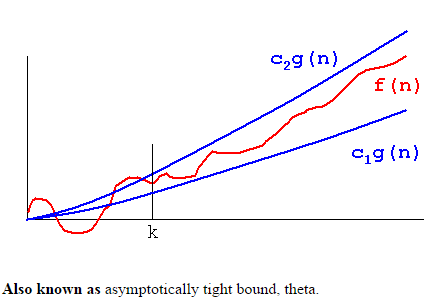
\includegraphics[width=0.6\linewidth]{BigTheta}

\end{figure}
Big-O is an upper bound for a function and Big-Omega is a lower-bound.  If the two bounds agree, then the function is sandwiched and is Big-theta of the common function.
\end{frame}
\begin{frame}
\large
\textbf{Do not confuse!}
	
	Not to be confused with worst, best and average cases analysis: all three (Omega, O, Theta) notation are not related to the best, worst and average cases analysis of algorithms. Each one of these can be applied to each analysis.
\end{frame}
%==================================%
\end{document}
